\section{Results}
\label{sec:results}

\para{Main comparison.}
\Tabref{tab:main_results} reports validation-selected layers and held-out test performance. The layer-local \itl selects layer 5 and reaches 19.53\% test top-1 accuracy, compared with 12.50\% for \finalmajority and 0.78\% for \majorityword. Among learned whole-word methods, \itl also has the best validation top-1, test top-1, and test MRR. \rawproto reaches a higher test top-5 accuracy at its selected layer, but its top-1 accuracy remains 5.47 points below \itl.

\begin{table}[t]
    \centering
    \caption{Validation-selected whole-word retrieval results. Higher is better for all metrics. Best comparable values in each metric column are in \textbf{bold}.}
    \label{tab:main_results}
    \resizebox{\textwidth}{!}{%
    \begin{tabular}{@{}lcccc@{}}
        \toprule
        \textbf{Method} & \textbf{Selected layer} & \textbf{Validation top-1} & \textbf{Test top-1} & \textbf{Test top-5 / MRR} \\
        \midrule
        \methodname & 5 & \textbf{21.09\%} & \textbf{19.53\%} & 25.59\% / \textbf{0.240} \\
        \finalmajority & -- & 12.50\% & 12.50\% & -- / -- \\
        \rawproto & 22 & 11.33\% & 14.06\% & \textbf{29.69\%} / 0.220 \\
        \meansubtok & 0 & 8.59\% & 10.94\% & 21.88\% / 0.175 \\
        \ridgeitl & 17 & 6.25\% & 3.71\% & 11.52\% / 0.092 \\
        \majorityword & -- & 0.78\% & 0.78\% & -- / -- \\
        \bottomrule
    \end{tabular}
    }
\end{table}


\para{Statistical evidence.}
\Tabref{tab:stat_tests} shows paired test-set comparisons. The primary comparison is \itl layer 5 versus \finalmajority. The accuracy difference is +7.03 percentage points with bootstrap \ci [2.53, 11.72], paired randomization $p=0.0045$, and McNemar exact $p=0.0046$. The selected \itl also beats \rawproto layer 22 by +5.47 points and \meansubtok layer 0 by +8.59 points, with positive confidence intervals in both cases.

\begin{table}[t]
    \centering
    \caption{Paired test-set comparisons for top-1 accuracy. Differences are \itl minus the comparison method. Confidence intervals are paired bootstrap intervals.}
    \label{tab:stat_tests}
    \resizebox{\textwidth}{!}{%
    \begin{tabular}{@{}lcccc@{}}
        \toprule
        \textbf{Comparison} & \textbf{Accuracy diff.} & \textbf{Bootstrap \ci} & \textbf{Randomization $p$} & \textbf{McNemar $p$} \\
        \midrule
        \itl layer 5 vs. \finalmajority & +7.03 pp & [2.53, 11.72] pp & 0.0045 & 0.0046 \\
        \itl layer 5 vs. \rawproto layer 22 & +5.47 pp & [2.15, 8.79] pp & 0.0023 & 0.0020 \\
        \itl layer 5 vs. \meansubtok layer 0 & +8.59 pp & [5.08, 12.11] pp & $<0.001$ & $<0.001$ \\
        \bottomrule
    \end{tabular}
    }
\end{table}


\para{Layer-wise behavior.}
\Figref{fig:layerwise} shows how retrieval quality changes by layer. \itl rises quickly and peaks at layer 5, then declines gradually. \rawproto peaks much later, at layer 22, which suggests that final-layer prototypes are geometrically best matched to late states. The explicit final-subtoken diagnostic is strongest at layer 0, with 20.12\% test accuracy over the 16 suffix IDs, and falls in early and middle layers while word-level \itl improves. This pattern is qualitatively consistent with token erasure: surface suffix identity becomes less directly recoverable as a whole-word representation becomes more decodable.

\begin{figure}[t]
    \centering
    \begin{minipage}[t]{0.48\linewidth}
        \centering
        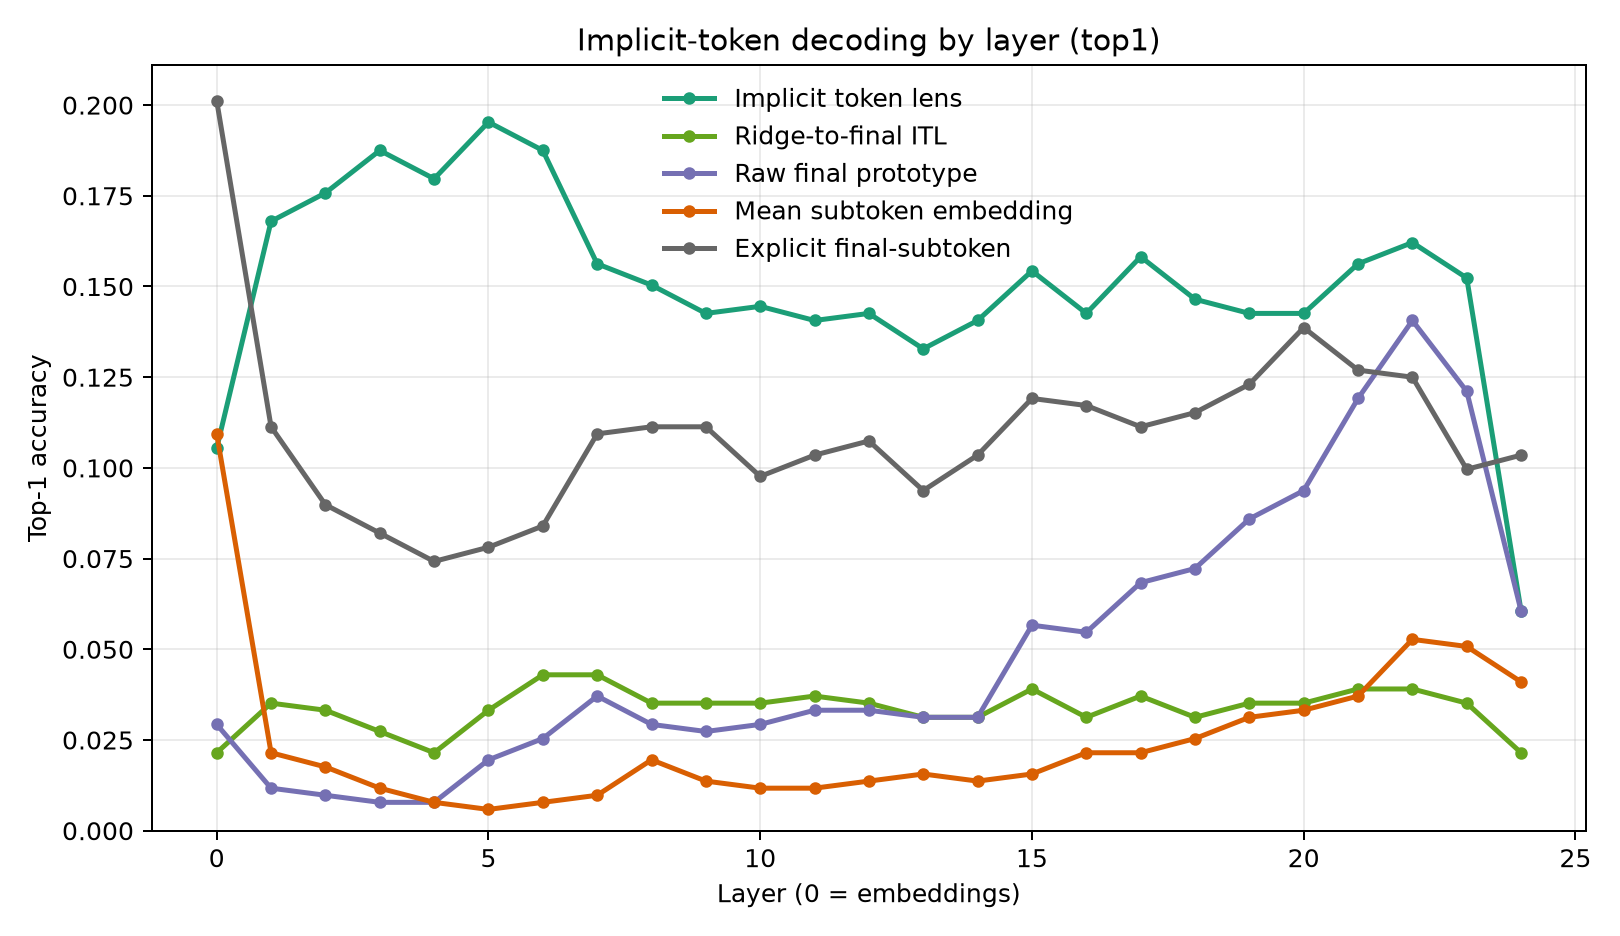
\includegraphics[width=\linewidth]{figures/layer_top1_accuracy.png}\\[-2pt]
        {\small (a) Top-1 accuracy}
    \end{minipage}
    \hfill
    \begin{minipage}[t]{0.48\linewidth}
        \centering
        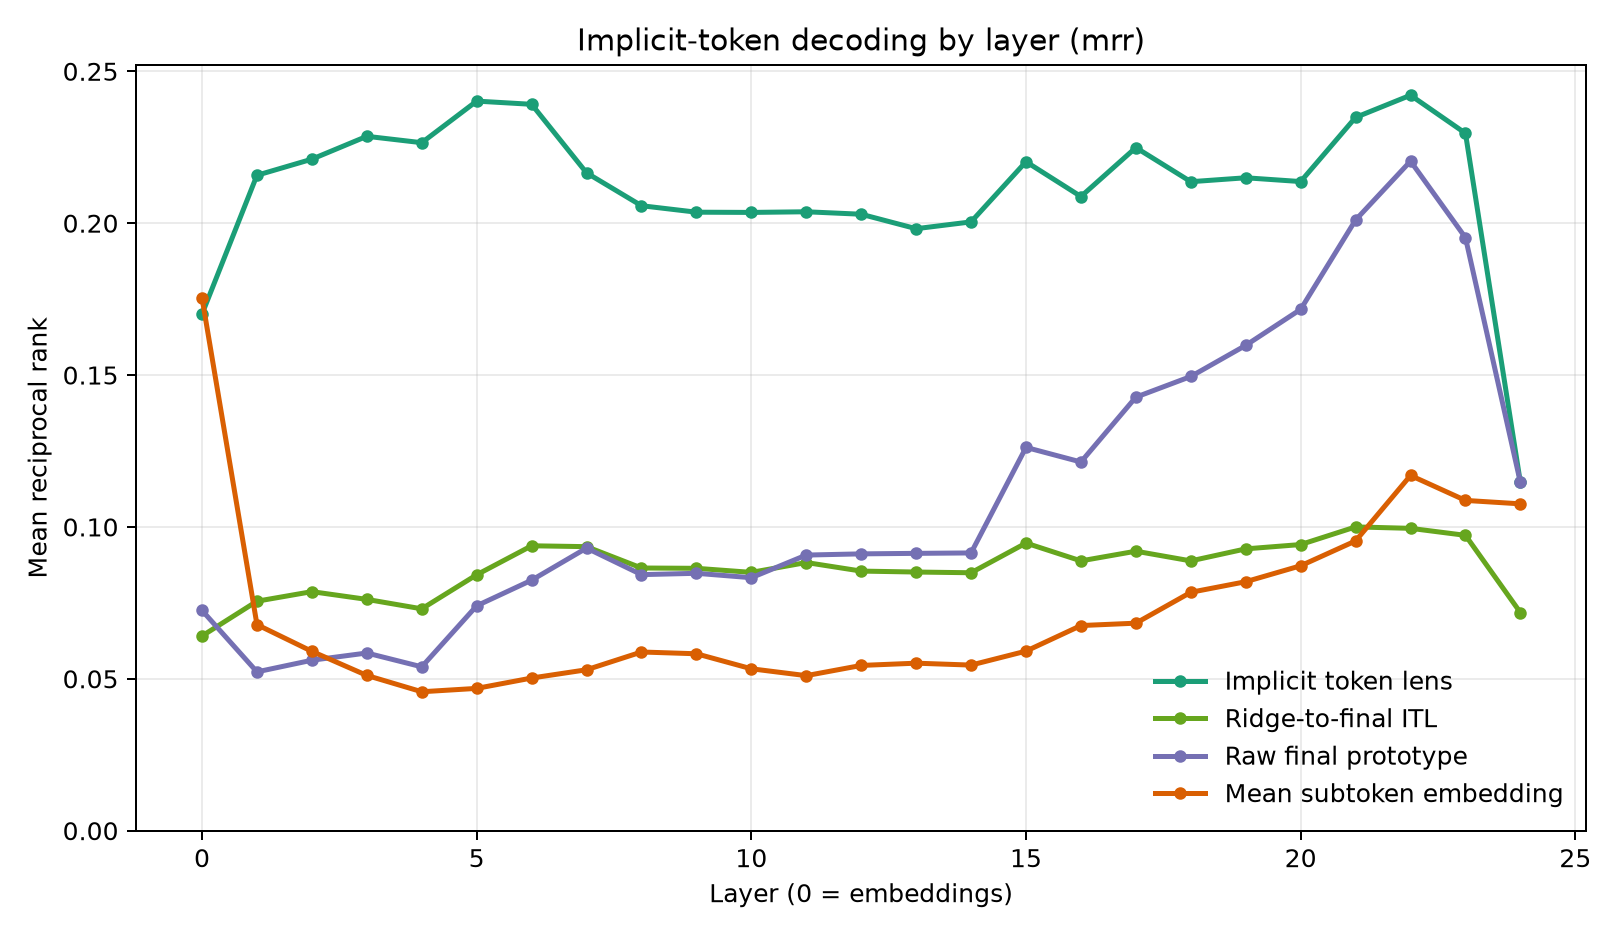
\includegraphics[width=\linewidth]{figures/layer_mrr.png}\\[-2pt]
        {\small (b) Mean reciprocal rank}
    \end{minipage}
    \caption{Layer-wise decoding results on validation and test splits. \itl peaks early at layer 5, while the raw final-prototype baseline is strongest late in the model. The final-subtoken diagnostic measures suffix-token recovery rather than whole-word retrieval.}
    \label{fig:layerwise}
\end{figure}

\para{Ablation: translating to final prototypes is weak.}
The ridge-to-final ablation is the closest analogue to the \tunedlens idea in this experiment: map each layer into a fixed final-layer prototype space, then decode against that table. It performs poorly, selecting layer 17 by validation top-1 and reaching only 3.71\% test top-1. This does not show that affine translators cannot work in principle. It does show that with 10 training occurrences per word and 896-dimensional states, the simple ridge translator is a poor fit compared with layer-local prototype rows.

\para{Error analysis.}
\Tabref{tab:error_examples} gives representative failures. Many mistakes stay inside the same final-subtoken group, such as `england' decoded as `highland' or `queensland'. However, not all errors are suffix-only: one `ireland' occurrence is ranked second as `lebanon'. The failures suggest that the hidden state mixes whole-word identity with residual orthographic information and contextual semantics. This is also why the final-subtoken control is important: \itl improves over suffix identity, but suffix and topic remain substantial confounds.

\begin{table}[t]
    \centering
    \caption{Representative \itl layer-5 errors on held-out examples. Some failures preserve the final tokenizer piece, while others reflect contextual or semantic confusions beyond the suffix group.}
    \label{tab:error_examples}
    \begin{tabular}{@{}llcl@{}}
        \toprule
        \textbf{Target} & \textbf{Prediction} & \textbf{Rank} & \textbf{Shared final token} \\
        \midrule
        england & highland & 10 & yes (`land') \\
        ireland & lebanon & 2 & no \\
        england & queensland & 114 & yes (`land') \\
        \bottomrule
    \end{tabular}
\end{table}

